\documentclass[a4paper,12pt]{article}

\usepackage[utf8]{inputenc}
\usepackage[italian]{babel}
\usepackage{graphicx}
\usepackage{float}

\title{Final Project Reti Logiche 2019}
\author{Lichinchi Federico, Lorenzi Davide}

\makeindex

\begin{document}
\maketitle
\newpage
\tableofcontents
\newpage

Qui di seguito verranno descritti nel dettaglio il problema da risolvere, le scelte progettuali relative alla macchina, i test creati e i relativi risultati e infine i risultati della sintesi.

\section{Descrizione del problema}
Viene fornito uno spazio bidimensionale definito in termini di dimensione orizzontale e verticale, e siano date le posizioni di N punti, detti “centroidi”, appartenenti a tale spazio. Si vuole implementare un componente HW descritto in VHDL che, una volta fornite le coordinate di un punto appartenente a tale spazio, sia in grado di valutare a quale/i dei centroidi risulti più vicino (Manhattan distance).
Lo spazio in questione è un quadrato (256x256) e le coordinate nello spazio dei centroidi e del punto da valutare sono memorizzati in una memoria (la cui implementazione non è parte del progetto). La vicinanza al centroide viene espressa tramite una maschera di bit (maschera di uscita) dove ogni suo bit corrisponde ad un centroide: il bit viene posto a 1 se il centroide è il più vicino al punto fornito, 0 negli altri casi. Nel caso il punto considerato risulti equidistante da 2 (o più) centroidi, i bit della maschera d’uscita relativi a tali centroidi saranno tutti impostati ad 1.
Degli N centroidi K $\leq$ N sono quelli su cui calcolare la distanza dal punto dato. I K centroidi sono indicati da una maschera di ingresso a N bit: il bit a 1 indica che il centroide è da valutare, mentre il bit a 0 indica che il centroide non deve essere esaminato. Si noti che la maschera di uscita è sempre a N bit e che i bit a 1 saranno non più di K.

\section{Specifiche del progetto}
Nella progettazione della macchina si sono tenute conto le seguenti specifiche.

\subsection{Interfaccia del componente}
Il componente da descrivere deve avere un'interfaccia composta dai seguenti segnali:
\begin{itemize}
\item \texttt{i\_clk} è il segnale di CLOCK in ingresso generato dal TestBench;
\item \texttt{i\_start} è il segnale di START generato dal Test Bench;
\item \texttt{i\_rst} è il segnale di RESET che inizializza la macchina pronta per ricevere il primo segnale di START;
\item \texttt{i\_data} è il segnale (vettore) che arriva dalla memoria in seguito ad una richiesta di lettura;
\item \texttt{o\_address} è il segnale (vettore) di uscita che manda l’indirizzo alla memoria;
\item \texttt{o\_done} è il segnale di uscita che comunica la fine dell’elaborazione e il dato di uscita scritto in memoria;
\item \texttt{o\_en} è il segnale di ENABLE da dover mandare alla memoria per poter comunicare (sia in lettura che in scrittura);
\item \texttt{o\_we} è il segnale di WRITE ENABLE da dover mandare alla memoria (=1) per poter scriverci. Per leggere da memoria esso deve essere 0;
\item \texttt{o\_data} è il segnale (vettore) di uscita dal componente verso la memoria.
\end{itemize}
\subsection{La RAM}
L'architettura della RAM, su cui si trovano le coordinate dei centroidi e la bit-mask, non viene istanziata nella macchina, dato che è già presente nel Test Bench. Le coordinate e la bit-mask sono salvate nei primi 18 indirizzi di memoria e codificati a 8 bit. 

Questi valori non vengono modificati per tutta l'esecuzione del codice. La macchina scriverà il risultato della computazione all'indirizzo 19 della RAM. Ulteriori indirizzi della RAM non possono essere utilizzati per la computazione.
\subsection{Il Clock}
La macchina deve funzionare con un clock di 100 ns.
\subsection{Sintesi e simulazione}
Il codice VHDL non deve presentare errori di compilazione. Il componente dev'essere almeno descritto e simulabile correttamente in pre-sintesi. Per raggiungere l'eccellenza nella risoluzione del progetto si richiede che il componente sia sintetizzabile e simulabile anche in post-sintesi.


\section{Scelte progettuali}
Per la risoluzione del problema assegnato si è deciso di procedere con l'ideazione e l'implementazione di una macchina a stati. La macchina consta 12 stati, numerati da 0 a 10 e uno stato di reset. 
Per il calcolo della distanza è stata utilizzata la formula della "Manhattan distance".

La macchina è classificabile come macchina di Moore in quanto le uscite dipendono solamente dallo stato corrente.

Onde evitare errori in lettura o in scrittura dei dati durante la Timing Simulation, si è deciso di attendere un interno ciclo di clock prima di ricevere o scrivere il dato richiesto, ottenendo informazioni solo sul fronte di salita.

\subsection{Segnali}
Come prima cosa, son stati definiti due tipologie di segnale:
\begin{itemize}
\item \textbf{STATO}: utilizzato per definire gli stati della macchina;
\item \textbf{D\_ARRAY}: utilizzato per definire un array di 8 segnali definiti da 9 bit, in quanto la massima distanza misurabile tra due centroidi è di 510 bit.
\end{itemize}
I segnali utilizzati dalla macchina sono stati:
\begin{itemize}
\item \texttt{distances}(D\_ARRAY): usato per memorizzare tutte le 8 distanze calcolate;
\item \texttt{minDistance}(unsigned): usato per memorizzare la distanza minima calcolata;
\item \texttt{currState}(STATO): usato per memorizzare lo stato in esecuzione;
\item \texttt{nextState}(STATO): usato per memorizzare il prossimo stato della macchina;
\item \texttt{prevState}(STATO): usato per memorizzare il prossimo stato della macchina da eseguire successivamente allo stato di lettura del dato dalla RAM;
\item \texttt{bitMask}(std\_logic\_vector):usato per memorizzare la bit-mask che la macchina legge dall'indirizzo 0 della RAM;
\item \texttt{Xc}(signed): usato per memorizzare l'ascissa del punto da valutare, che la macchina legge dall'indirizzo 17 della RAM;
\item \texttt{Yc}(signed): usato per memorizzare l'ordinata del punto da valutare, che la macchina legge dall'indirizzo 18 della RAM;
\item \texttt{Xp}(signed): usato per memorizzare l'ascissa del centroide considerato nel calcolo;
\item \texttt{Yp}(signed): usato per memorizzare l'ordinata del centroide considerato nel calcolo;
\item \texttt{maskPtr}(integer): usato come contatore per scorrere lungo la bit-mask;
\item \texttt{cntrPtr}(integer): usato come contatore per cambiare l'indirizzo di lettura della RAM;
\item \texttt{outMask}(std\_logic\_vector): usato per memorizzare la maschera di uscita da scrivere nella RAM.
\end{itemize}
Tutti i segnali sopraelencati, a eccezione dei segnali \texttt{currState, nextState, i\_start, i\_rst, i\_data e i\_clk}, hanno un omonimo segnale con prefisso next per mantenere memorizzato il loro valore nel ciclo successivo.

\subsection{Stati}
La macchina è composta dai seguenti stati:
\begin{itemize}
\item \texttt{RST}: stato di reset, in cui vengono ripristinati al valore iniziale i segnali coinvolti nell'elaborazione. Si entra in questo stato quando \texttt{i\_rst} va a '1' oppure prima di iniziare la computazione;
\item \texttt{S0}: stato di idle, in cui si aspetta che i\_start vada a '1' per poter cominciare l'elaborazione. L'elaborazione comincia dallo stato \texttt{RST};
\item \texttt{S1}: in questo stato si assegnano i parametri per la lettura della bit-mask;
\item \texttt{S2}: in questo stato si salva la bit-mask appena letta e si assegnano i parametri per la lettura dell'ascissa del punto da valutare;
\item \texttt{S3}: in questo stato si salva l'ascissa del punto da valutare e si assegnano i parametri per la lettura dell'ordinata del punto da valutare;
\item \texttt{S4}: in questo stato si salva l'ordinata del punto da valutare, si assegnano i parametri per la lettura dell'ascissa del primo centroide;
\item \texttt{S5}: in questo stato si salva l'ascissa del centroide considerato e si assegnano i parametri per la lettura dell'ordinata del centroide stesso;
\item \texttt{S6}: in questo stato si salva l'ordinata del centroide considerato, si calcola la distanza di Manhattan e la si assegna a \texttt{distance}, tramite l'ausilio di funzioni matematiche (\texttt{abs}). Noi abbiamo calcolato la distanza in un'unica equazione, senza aver progettato alcun blocco logico, in quanto questo porterebbe complicazioni nell'implementazione. Una volta calcolata la distanza, la confrontiamo con la \texttt{min\_distance}. Se \texttt{min\_distance} risulta maggiore, allora va aggiornato il suo valore. Successivamente \texttt{distance} va salvata in \texttt{distances}. Se abbiamo letto tutti i centroidi, si va allo stato \texttt{S7}, altrimenti si ritorna in \texttt{S5} e si continua con la lettura dell'ascissa del centroide successivo;
\item \texttt{S7}: in questo stato si confrontano tutte le distanze calcolate con la distanza minima. Se la distanza calcolata in un centroide è uguale alla distanza minima, viene assegnato il valore '1' in \texttt{outMask} in corrispondenza del centroide considerato, altrimenti viene assegnato il valore '0'. Una volta ricavata la \texttt{outMask}, si assegnano i parametri per la scrittura della maschera di uscita all'indirizzo 19 della RAM;
\item \texttt{S8}: in questo stato si setta il segnale di \texttt{o\_done} a '1' e si assegnano i parametri per rimanere in attesa che il segnale \texttt{i\_start} vada a '0';
\item \texttt{S9}: in questo stato si abilita la RAM per la lettura o per la scrittura del dato;
\item \texttt{S10}: in questo stato si disabilita l'accesso alla RAM e non si cambia stato finché il segnale \texttt{i\_start} non va a '0'. Nel momento in cui ciò avviene, si ritorna nello stato di idle.
\end{itemize}

\subsection{Processi}
La macchina utilizza due processi in modo asincrono:
\begin{itemize}
\item \texttt{delta\_lambda}: in questo processo viene svolta l'intera computazione, e sono descritti tutti gli stati operativi della macchina;
\item \texttt{state}: questo processo coordina la propagazione dei segnali e la successione degli stati. In qualsiasi stato di elaborazione della macchina, il processo interviene ripristinando la macchina alle condizioni iniziali se il segnale \texttt{i\_rst} viene innalzato a '1'.
\end{itemize}

\section{Test creati e relativi risultati}

\subsection{Test creati}
Per verificare la corretta descrizione del componente abbiamo proceduto alla creazione di 5 test bench (oltre a quello fornito dal docente) in cui sono stati testati i limiti della macchina:

\begin{enumerate}
\item \textbf{tb\_bitmask\_nulla}: la bit-mask è composta tutta da '0';
\item \textbf{tb\_centroide\_coincidente}: un centroide ha le stesse coordinate del punto dal valutare;
\item \textbf{tb\_centroidi\_tutti\_uguali}: tutti i centroidi da esaminare hanno le stesse coordinate;
\item \textbf{tb\_distanza\_massima}: un centroide si trova a distanza massima dal punto da valutare (punto e centroide in angoli opposti della "griglia" della RAM);
\item \textbf{tb\_distanze\_incrementali}: ogni centroide dista a una distanza minore dal punto rispetto al successivo centroide da considerare.
\end{enumerate}


Come modello di riferimento per la creazione dei test bench è stato utilizzato il \textbf{tb\_salice\_reti\_logiche} che ha permesso un'efficiente preparazione dei test e una totale assenza di errori nella descrizione della RAM e del componente. 

La procedura di testing applicata è stata di black-box in quanto i test sono stati generati a partire dalle specifiche fornite e non dal codice descrittivo VHDL prodotto.



\newpage
\subsection{Risultati ottenuti}
Qui sotto sono riportati le schermate delle waveform ottenute e della stampa "TEST PASSATO" nella console al termine della "Run All" del progetto in Timing Simulation, per ogni test bench usato.

\begin{enumerate}
\item \textbf{tb\_bitmask\_nulla}: la bit-mask è composta tutta da '0';

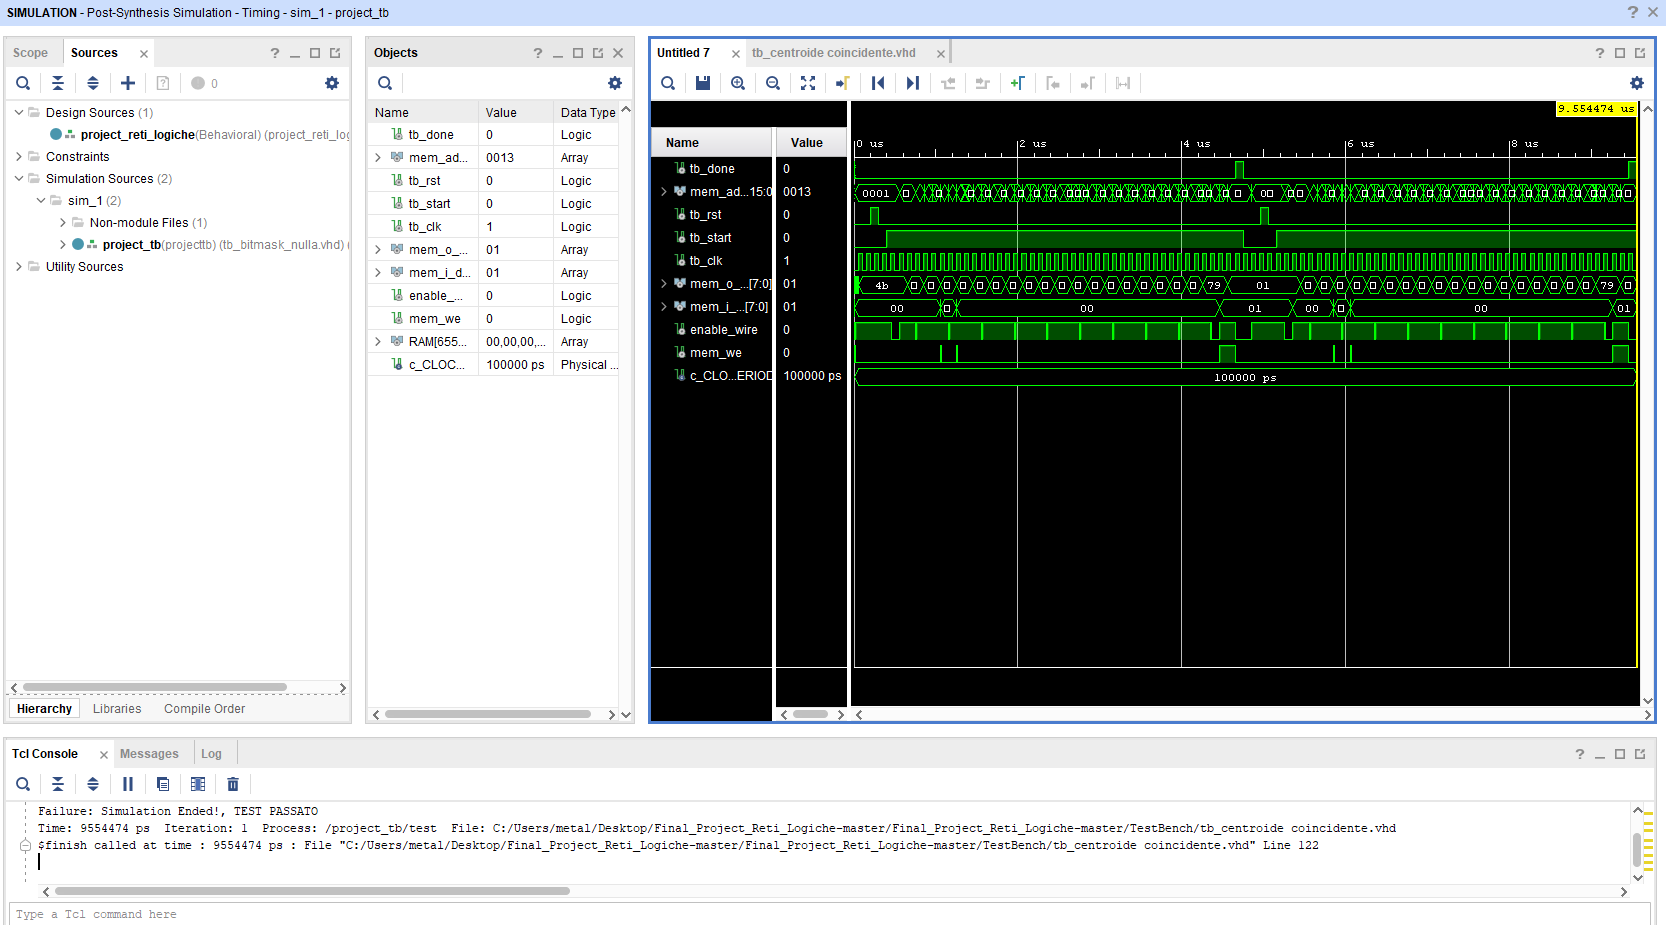
\includegraphics[scale=0.32]{images/tb_bitmask_nulla}

\item \textbf{tb\_centroide\_coincidente}: un centroide ha le stesse coordinate del punto dal valutare;

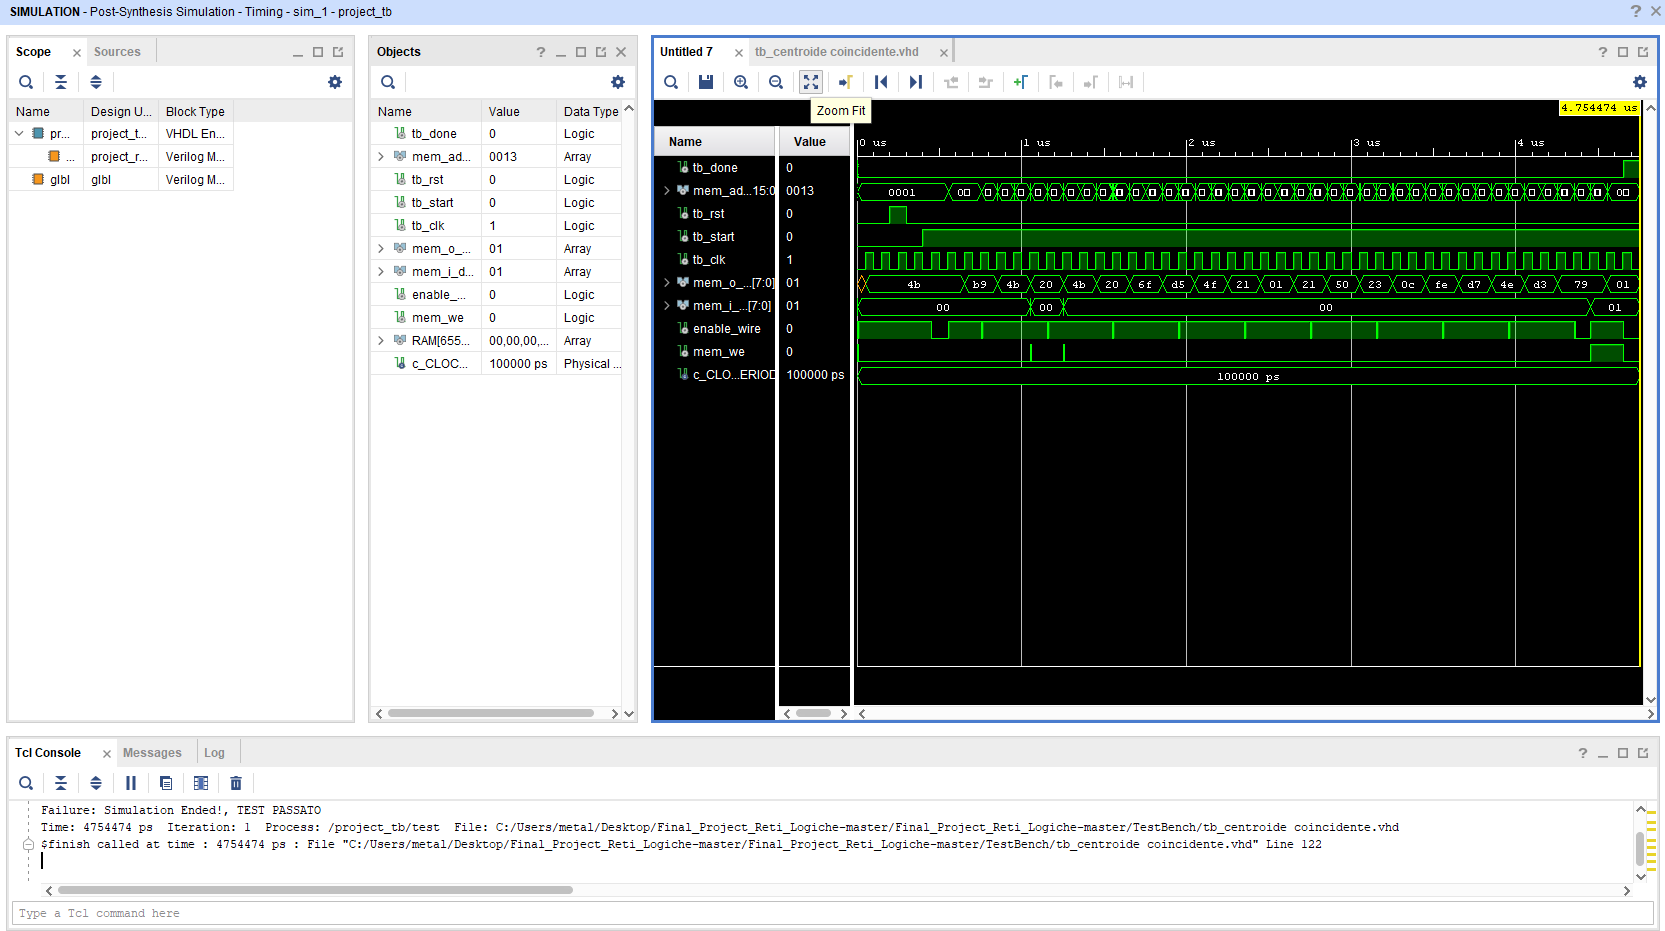
\includegraphics[scale=0.32]{images/tb_centroide_coincidente}

\newpage
\item \textbf{tb\_centroidi\_tutti\_uguali}: tutti i centroidi da esaminare hanno le stesse coordinate;

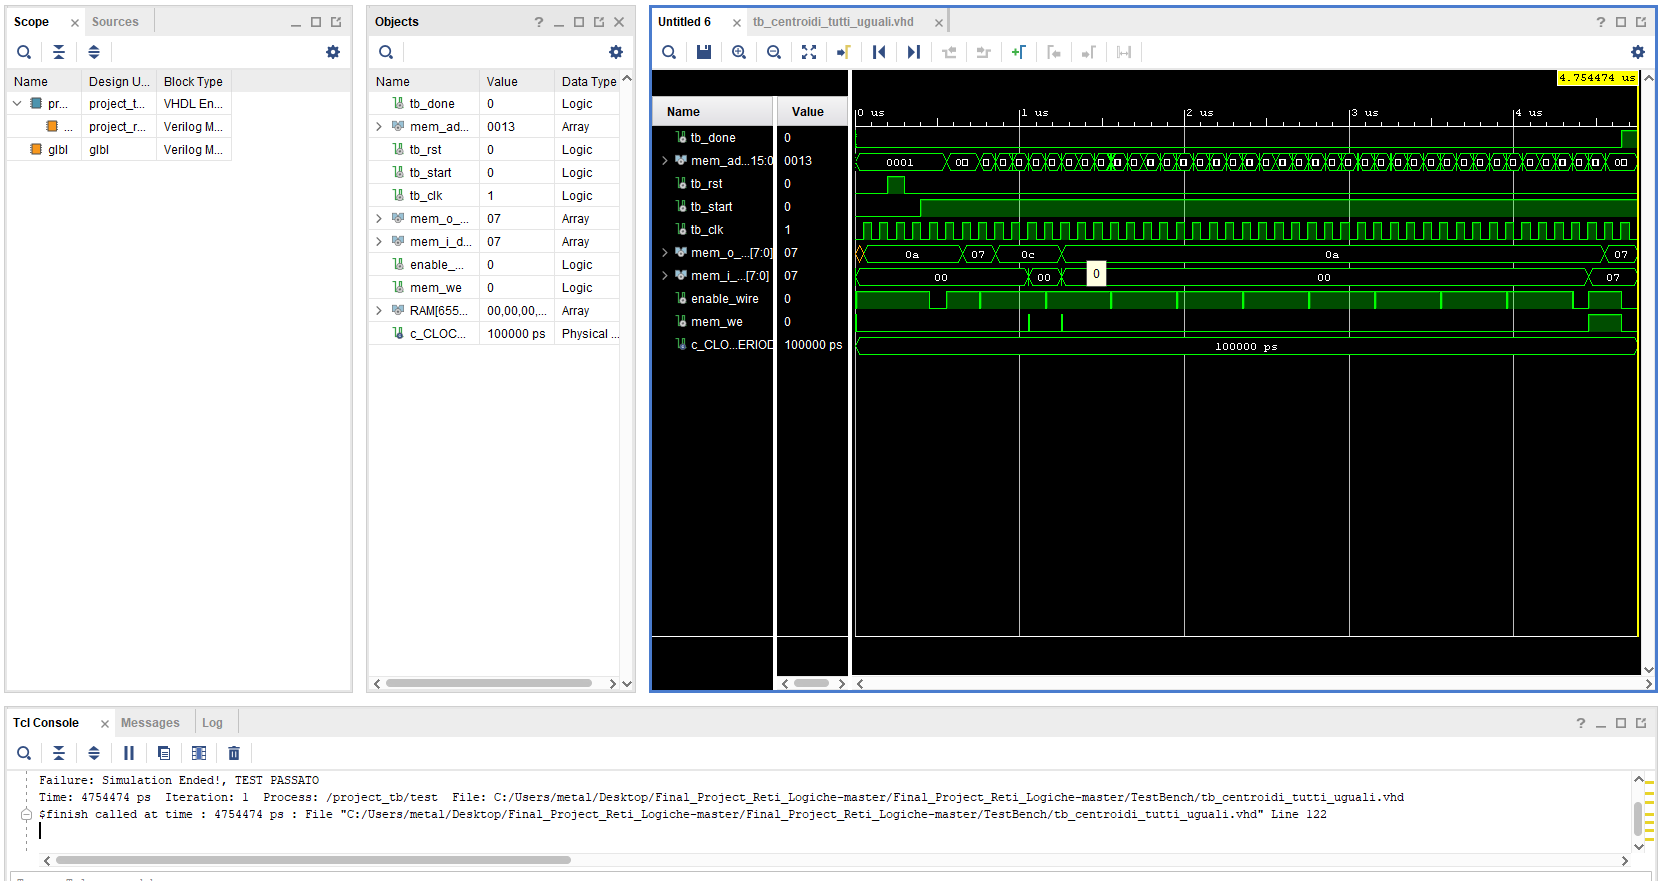
\includegraphics[scale=0.32]{images/tb_centroidi_tutti_uguali}

\item \textbf{tb\_distanza\_massima}: un centroide si trova a distanza massima dal punto da valutare (punto e centroide in angoli opposti della "griglia" della RAM);

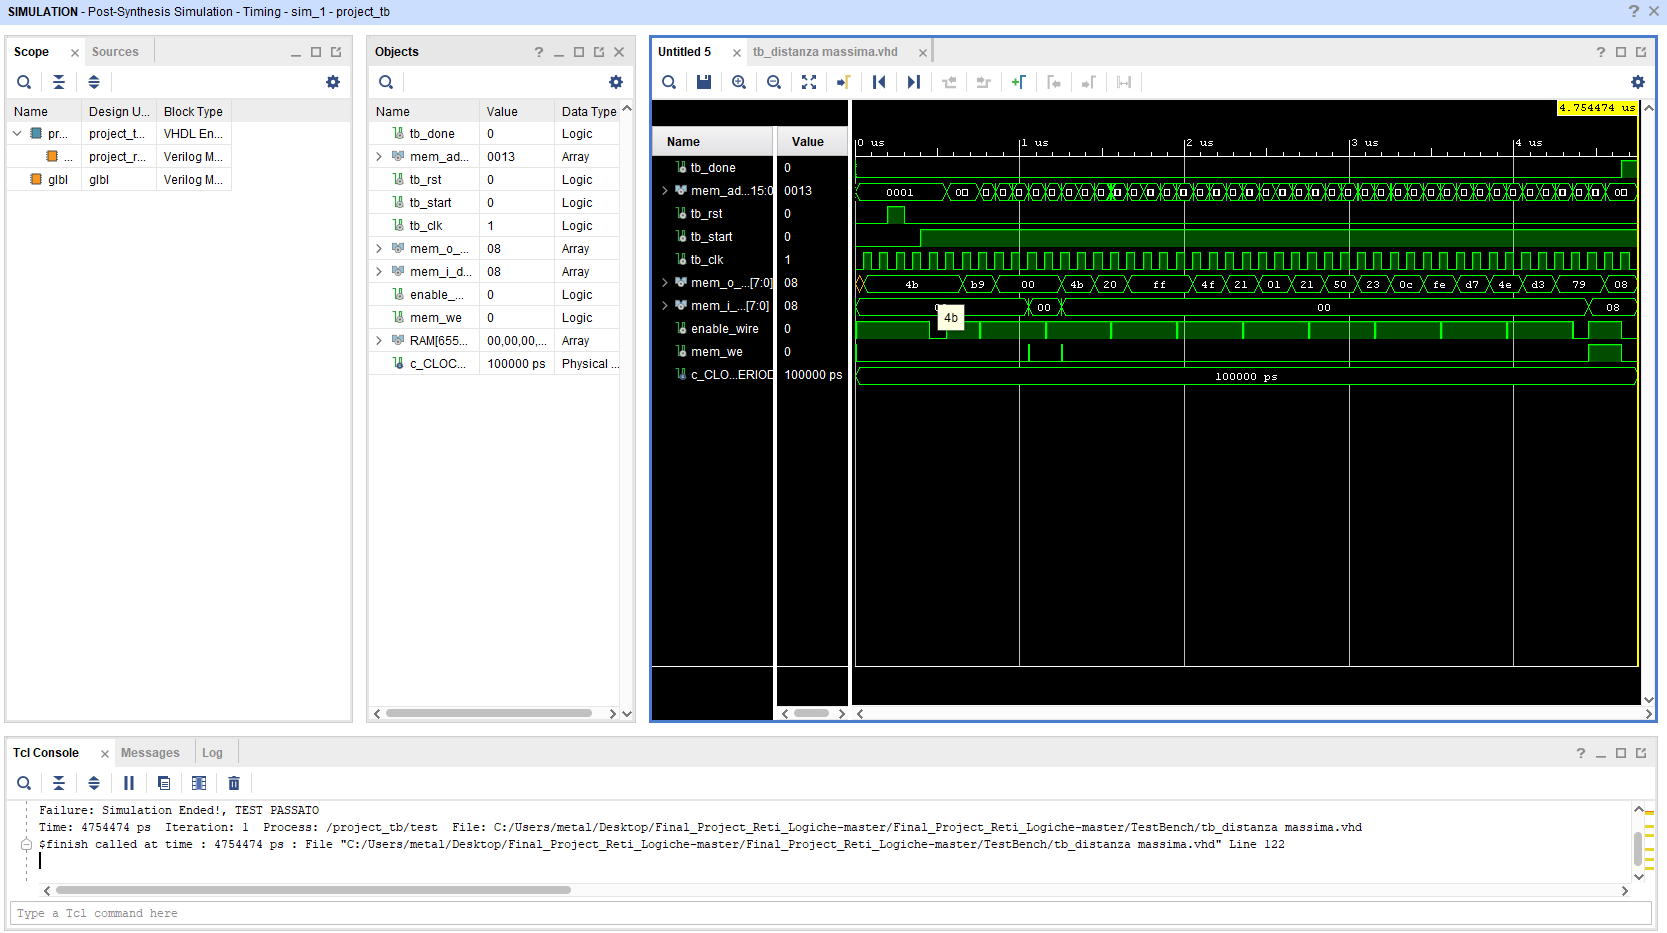
\includegraphics[scale=0.32]{images/tb_distanza_massima}

\newpage
\item \textbf{tb\_distanze\_incrementali}: ogni centroide dista a una distanza minore dal punto rispetto al successivo centroide da considerare.

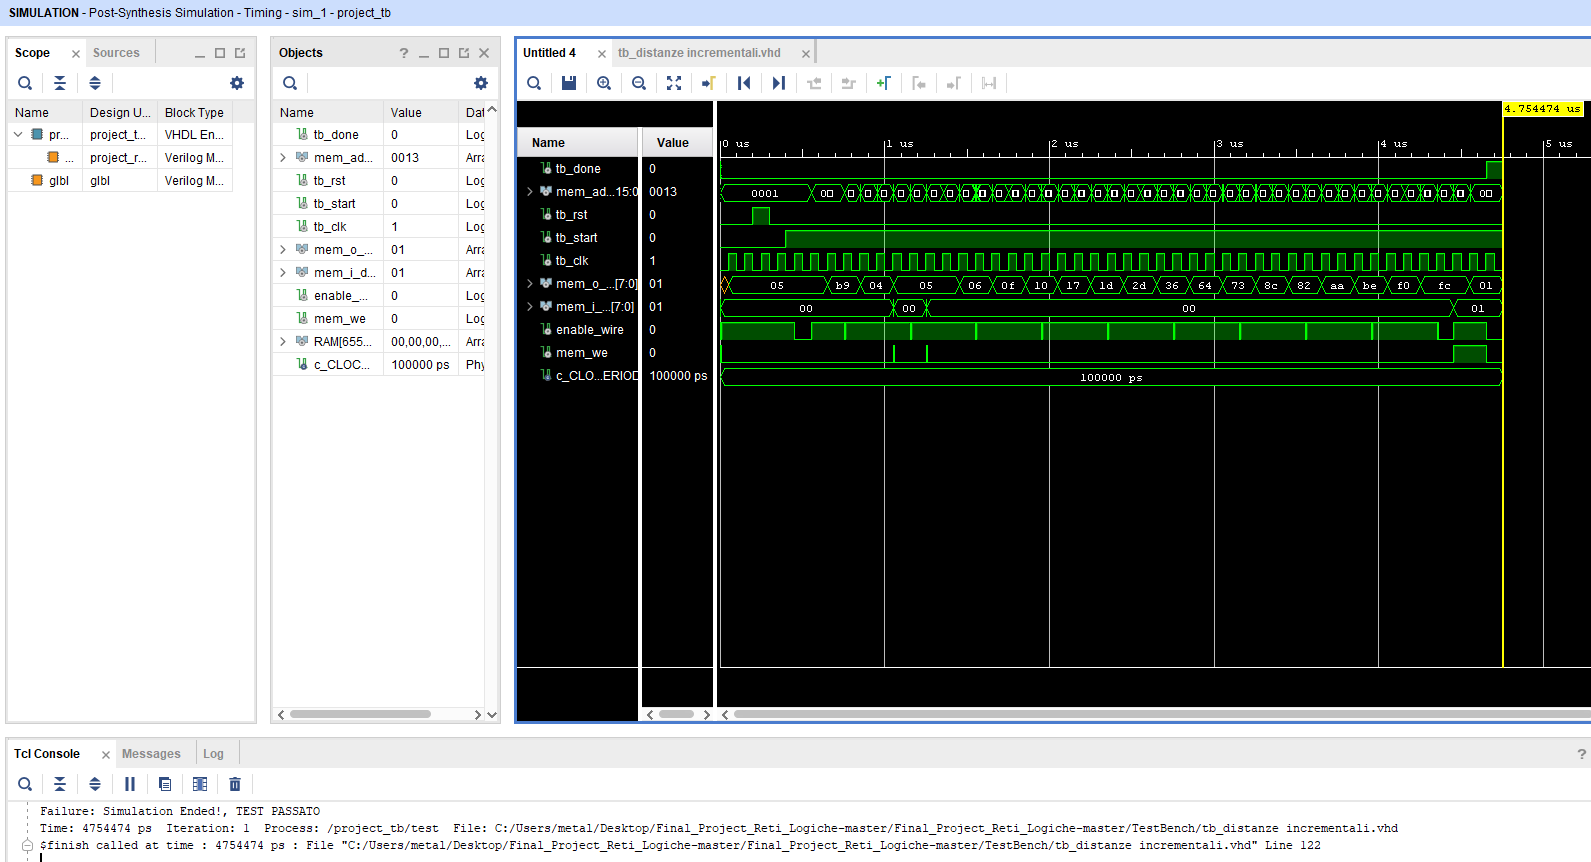
\includegraphics[scale=0.32]{images/tb_distanze_incrementali}

\item \textbf{tb\_salice\_reti\_logiche}: test bench fornito dal docente.

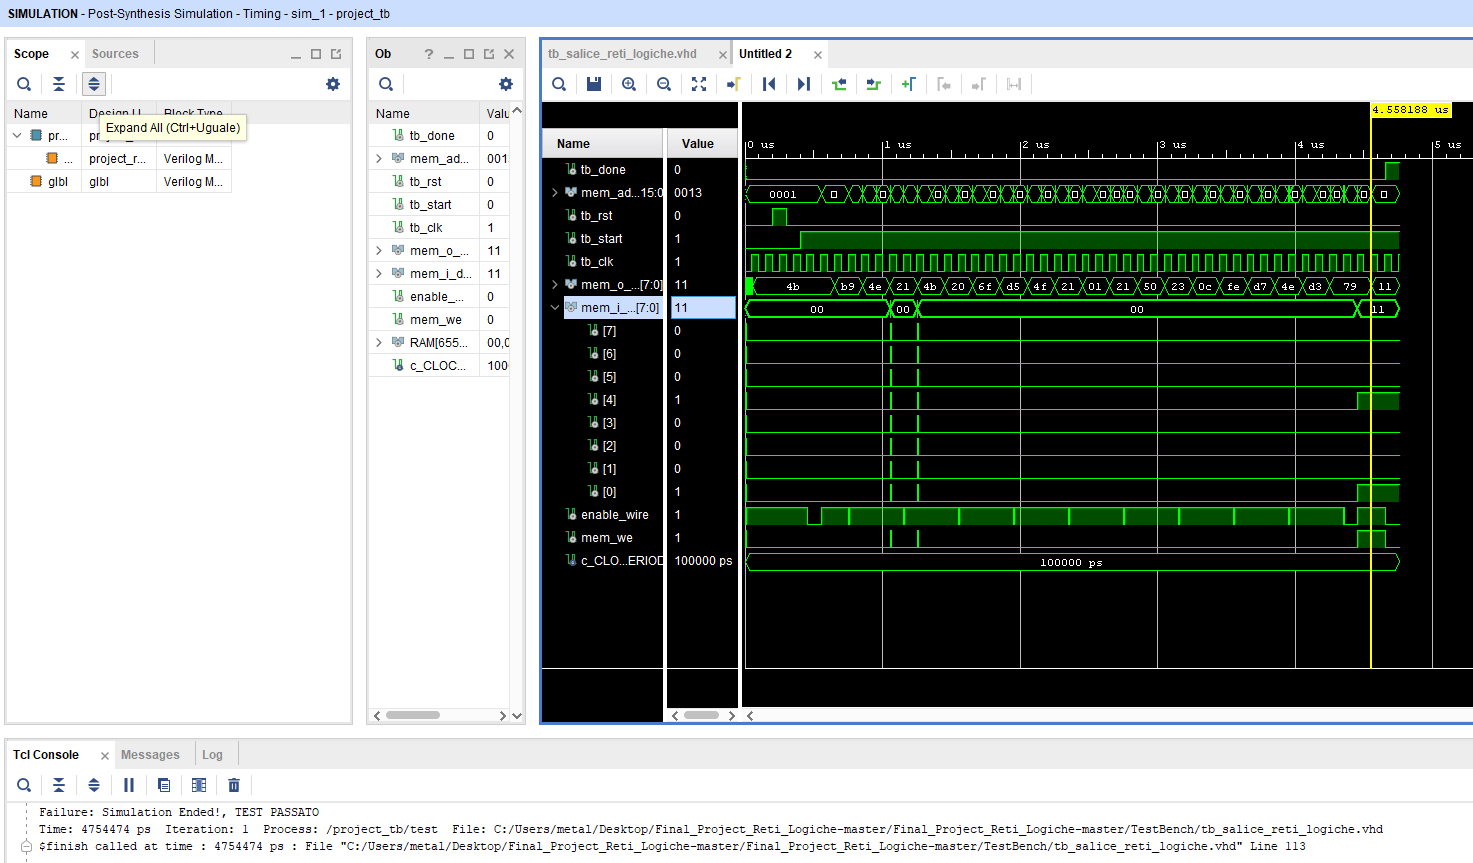
\includegraphics[scale=0.32]{images/tb_salice_reti_logiche}

\end{enumerate}

\section{Risultati sintesi}
Il componente descritto viene sintetizzato con successo, senza warning significanti che possono compromettere il corretto funzionamento (no inferring latch). Come dimostrato dalla sezione precedente, le simulazioni hanno dato esito positivo sia in pre-sintesi sia in post-sintesi (con timing).

\end{document}